\section{Introduction}
This chapter discusses the challenges encountered during the implementation of the project, and the limitations of the current project and possible future works.


\section{Challenges}
The researchers encountered a variety of challenges during the implementation of the project. These challenges are discussed below.

\begin{itemize}
    \item During the interviews, the researchers were not granted some information about the current system for confidentiality purposes. Information such as the detailed costs of the current system, revenue generated by the current system, and the number of tickets issued per day were not disclosed.
    \item Execution of the project was also dependent on funding to purchase equipment such as the microcontroller and servo motors which can easily be damaged by power surges.
    \item Majority of the respondents were regular(daily) users of the system and most especially students, leading to some bias in the information gathered. The researchers did not receive a significant number of responses from individuals within the occasional users category as well as university staff.
\end{itemize}


\section{Project Gaps and Future Works}
Currently, implementation of the project is limited to the university scope and only accounts for users with smartphones with iOS and Android Operating Systems.

Additionally, the researchers were limited to building a demonstration of the project using a servo motor and not a real-world gate. There is a need for a further study where the low-cost esp32 cameras are used at a real world toll / parking gate.

This project can also easily be scaled to various places such as malls and hospitals, and extended to account for non-smartphone users.


\section{Conclusion}
  In conclusion, the research's primary objective was to a great extent. An initiative of this nature is worth investing in and taking to the next level of having it publicly available as it would address so many shortcomings in the system currently in place that would benefit various groups in the Makerere University community from students, lecturers and other staff while also generating revenue for the university.


\clearpage
\bibliographystyle{IEEEtran}
\bibliography{references}
\begin{appendices}
    \textbf{Interview Questions: Motorist}
    \begin{itemize}
        \item What are some of the challenges you have faced using Makerere's toll gates?
        \item Describe the process of payment for toll fee at the ticket stations.
        \item How frequently do you use the Makerere university gates?
        \item Motorists who misplace their tickets are expected to pay a fine of 50,000 UGX. Have you ever misplaced your ticket? If yes, how did you resolve the issue? What are your thoughts on the fine?
    \end{itemize}

    \textbf{Interview Questions: Toll Operator}
    \begin{itemize}
        \item What was the motivation behind putting in place this system?
        \item What challenges do you normally face when managing these gates?
        \item What are some solutions you've put in place to alleviate the challenges you've had?
        \item Do you believe cashless payments would ease your organisation's work?
    \end{itemize}


    \begin{figure}
        \begin{center}
            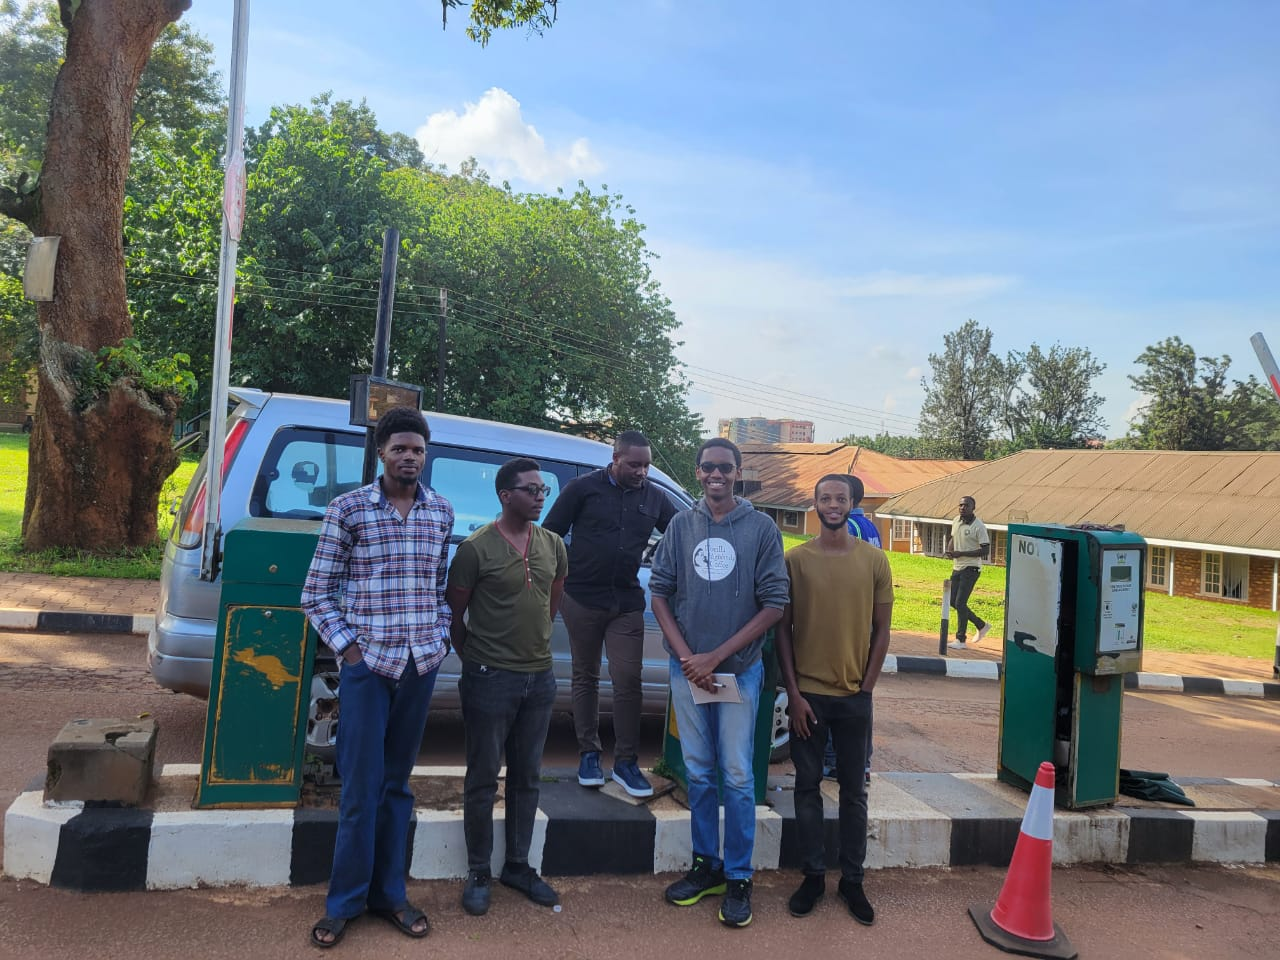
\includegraphics[scale = 0.3]{images/rizz.jpeg}
            \caption{The researchers also conducted in person interviews with motorists and the project manager at the toll gate}
        \end{center}
    \end{figure}
\end{appendices}